
% Este documento LaTeX fue diseñado por profesores  del Departamento de Matemáticas 
% de la Universidad de Antioqua (http://ciencias.udea.edu.co/). Usted puede modificarlo
% y personalizarlo a su gusto bajo los términos de la licencia de documentación libre GNU.
% http://es.wikipedia.org/w/index.php?title=Licencia_de_documentaci%C3%B3n_libre_de_GNU&oldid=15717448x

\documentclass[serif,9pt]{beamer}

\usetheme{Madrid}

%\documentclass[serif,9pt]{beamer}
%\usepackage[T1]{fontenc} % Needed for Type1 Concrete
%\usepackage[charter]{mathdesign}


%\usepackage[pdftex]{graphicx}
\usepackage[utf8]{inputenc}
\usepackage[latin1]{inputenc}
\usepackage[spanish]{babel}
\usepackage{enumerate}
\usepackage{graphicx}
\usepackage{verbatim}
\usepackage{subfig}
% Paquetes de la AMS:
\usepackage{amsmath, amsthm, amsfonts}
\usepackage[round, year]{natbib}  % Personalizar la bibliografía a gusto de cada quien
\bibliographystyle{unsrtnat}
 
\title{Bibliography management: \texttt{natbib} package}
\author{Share\LaTeX}
\date {}
% Teoremas
%--------------------------------------------------------------------------
\newtheorem{thm}{Teorema}[section]
\newtheorem{cor}[thm]{Corolario}
\newtheorem{lem}[thm]{Lema}
\newtheorem{prop}[thm]{Proposición}
\theoremstyle{definition}
\newtheorem{defn}[thm]{Definición}
\theoremstyle{remark}
\newtheorem{rem}[thm]{Observación}

%% (require 'iso-transl)
% Atajos.
% Se pueden definir comandos nuevos para acortar cosas que se usan
% frecuentemente. Como ejemplo, aquí se definen la R y la Z dobles que
% suelen representar a los conjuntos de números reales y enteros.
%--------------------------------------------------------------------------

\def\RR{\mathbb{R}}
\def\ZZ{\mathbb{Z}}
\begin{document}
\title[Presentaci\'on tesina]{Análisis de datos Géneticos Poblacional de Cáncer Colorrectal en México}
\author[Edison Vázquez]{Edison Vázquez}
\institute[CIMAT]{%
  Centro de Investigación en Matemáticas\\
  Unidad Monterrey}
\date[Marzo, 2018]


\begin{frame}
\titlepage
\end{frame}

\begin{frame}\frametitle{Contenido}\tableofcontents
\end{frame} 


\section{Avances}
\begin{frame}\frametitle{Avances y tareas por realizar}
  \linebreak
  TAREAS POR REALIZAR:
  \begin{itemize}
  \item Introducir las bases de datos obtenidas en la primera corrida del an\'alisis de ancestralidad y observar los mapas de calor de ancestralidad. \texttt{check}
  \item Revisar softwares que nos permitan recuperar regiones especificas en el genotipado de los datos.  \texttt{Check}
  \item Asociar las regiones de los SNP's con la ancestralidad de los individuos.\texttt{En proceso - 80\%}
  \end{itemize}
\end{frame}

\section{Estimaci\'on de ancestria}

\begin{frame}\frametitle{ADMIXTURE SOFTWARE}
  Varios autores han usado diferentes m\'etodos para la estimaci\'on de ancestr\'ia \cite{Vero,Justo,Nuri}. Los softwares de mayor uso, especificamente diseñados para realizar \textit{admixture mapping} en la literatura son los programas \texttt{STRUCTURE}, \texttt{MALDsoft}, \texttt{ADMIXMAP}, \texttt{ANCESTRYMAP} y \texttt{ADMIXTURE}. Este \'ultimo calcula las estimaciones mucho mas r\'apido usando un algoritmo n\'umerico de optimizaci\'on. Especificamente ADMIXTURE es una herramienta de software para la estimación de máxima verosimilitud de ancestros individuales de conjuntos de datos genotipo SNP multilocus. ADMIXTURE utiliza un enfoque de relajación de bloques (\textbf{block relaxation}) para actualizar alternativamente la frecuencia de alelos y los parámetros de la fracción ascendente. Cada actualización de bloques se maneja resolviendo una gran cantidad de problemas de optimización convexos independientes, que se abordan usando un algoritmo de programación cuadrático secuencial rápido. La convergencia del algoritmo se acelera utilizando un novedoso método de aceleración \textit{cuasi Newton}. El algoritmo supera a los algoritmos EM y los métodos de muestreo MCMC por un amplio margen \cite{Admixture}. Una vista general de los programas para la estimaci\'on de ancestria se puede observar en la tabla \ref{tabla:sofadm}. \\

\end{frame}

\begin{frame}\frametitle{ADMIXTURE SOFTWARE}

\begin{table}[htbp]
  \centering
\begin{tabular}[t]{|1|p{0.3\linewidth}|p{0.3\linewidth}|}
  \hline 
  \multicolumn{1}{|c|}{\textbf{Programa}} & \multicolumn{1}{c|}{\textbf{Global/local}} & \multicolumn{1}{c|}{\textbf{Sistema operativo}} \tabularnewline \hline
  STRUCTURE & Global/Local & Windows/Linux/Mac  \tabularnewline \hline
frappe &Global&	Windows/Linux/Mac \tabularnewline \hline
ADMIXTURE&Global&Linux/Mac \tabularnewline \hline
EIGENSTRAT/smartpca&Global&Linux\tabularnewline \hline
ipPCA/EigenDev&Global&Windows/Linux(MatLab) \tabularnewline \hline
GEMTools&Global&Windows/Linux \tabularnewline \hline
PLINK&Global&Windows/Linux/Mac/C/C++ \tabularnewline \hline
LAMP&Local/Global&Windows/Linux \tabularnewline \hline
SABER&Local/Global&Linux \tabularnewline \hline
HAPMIX&Local/Global&Unix/Linux/Windows \tabularnewline \hline
ANCESTRYMAP&Local/Global&Unix/Linux \tabularnewline \hline

\end{tabular}
\caption{Descripci\'on de programas  para la estimaci\'on de ancestria local o globlal \cite{Yushi}}
\label{tabla:sofadm}
\end{table}
\end{frame}


\begin{frame}\frametitle{ADMIXTURE SOFTWARE}
  
  A grandes rasgos, el programa ADMIXTURE estima la probabilidad para los genotipos observados basandose en las proporciones de ascedencia y frecuencias de alelos de poblaci\'on. Esto lo realiza simultaneamente, mientras estima las frecuencias de alelos de pobaci\'on lo hace junto a la estimaci\'on de las proporciones de ascedencia.\linebreak

  \begin{figure}[H]
  \centering
  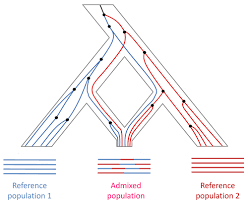
\includegraphics[scale=0.5]{images.png}
  \caption{ ``La figura muestra un árbol de población (en gris) y un árbol de genes (en azul y rojo) que rastrea la historia evolutiva de dos poblaciones ancestrales y su correspondiente población mezclada. Debido a ILS, los haplotipos específicos de la población de referencia 1 (líneas rojas) podrían fluir y mezclarse con la población 2 y viceversa.''  \cite{Yuan}}
  \label{fig:adm}
  \end{figure}
\end{frame}
  
  \begin{frame}\frametitle{ESTIMANDO EL MEJOR K}
    
    Para la estimaci\'on de la ancestr\'ia es necesario conocer apriori las poblaciones que existen dentro de la muestra. En este caso se usa el m\'etodo de \textit{cross-validation} para identificar el valor de \textbf{K}.  Este procedimiento divide los genotipos observados en v=5 (por defecto) folds de aproximadamente el mismo tamaño. El procedimiento enmascara (es decir, convierte a ``MISSING'') todos los genotipos, para cada fold a su vez. Osea, para cada fold, el conjunto enmascarado \ltilde{G} resultante es usado para calcular las estimaciones $\tilde{\theta}$ = ($\tilde{Q}$,$\tilde{P}$). \linebreak

    Ante este procedimiento se corri\'o el primer an\'alisis para estimar el n\'umero de poblaciones dentro de nuestros datos. \linebreak

    
\begin{table}[H]
\centering
\begin{tabular}{|1|1|1|}
  
\hline \hline
\# de poblaciones & \# de iteracciones & Tiempo de ejecuci\'on (min)\\
\hline
2 & 33 & 311\\
\hline
3 & 59 & 645\\
\hline
4 & 73 & 922 \\
\hline
5 & 94 & 1322\\
\hline
& TOTAL & 3200 (53 hrs.)\\

\hline \hline

\end{tabular}
\caption{Ejecuci\'on para la b\'usqueda del mejor K}
\label{tabla:K}
\end{table}

\end{frame}


\begin{frame}\frametitle{ESTIMANDO EL MEJOR K}
    
 
\begin{figure}[H]
  \centering
  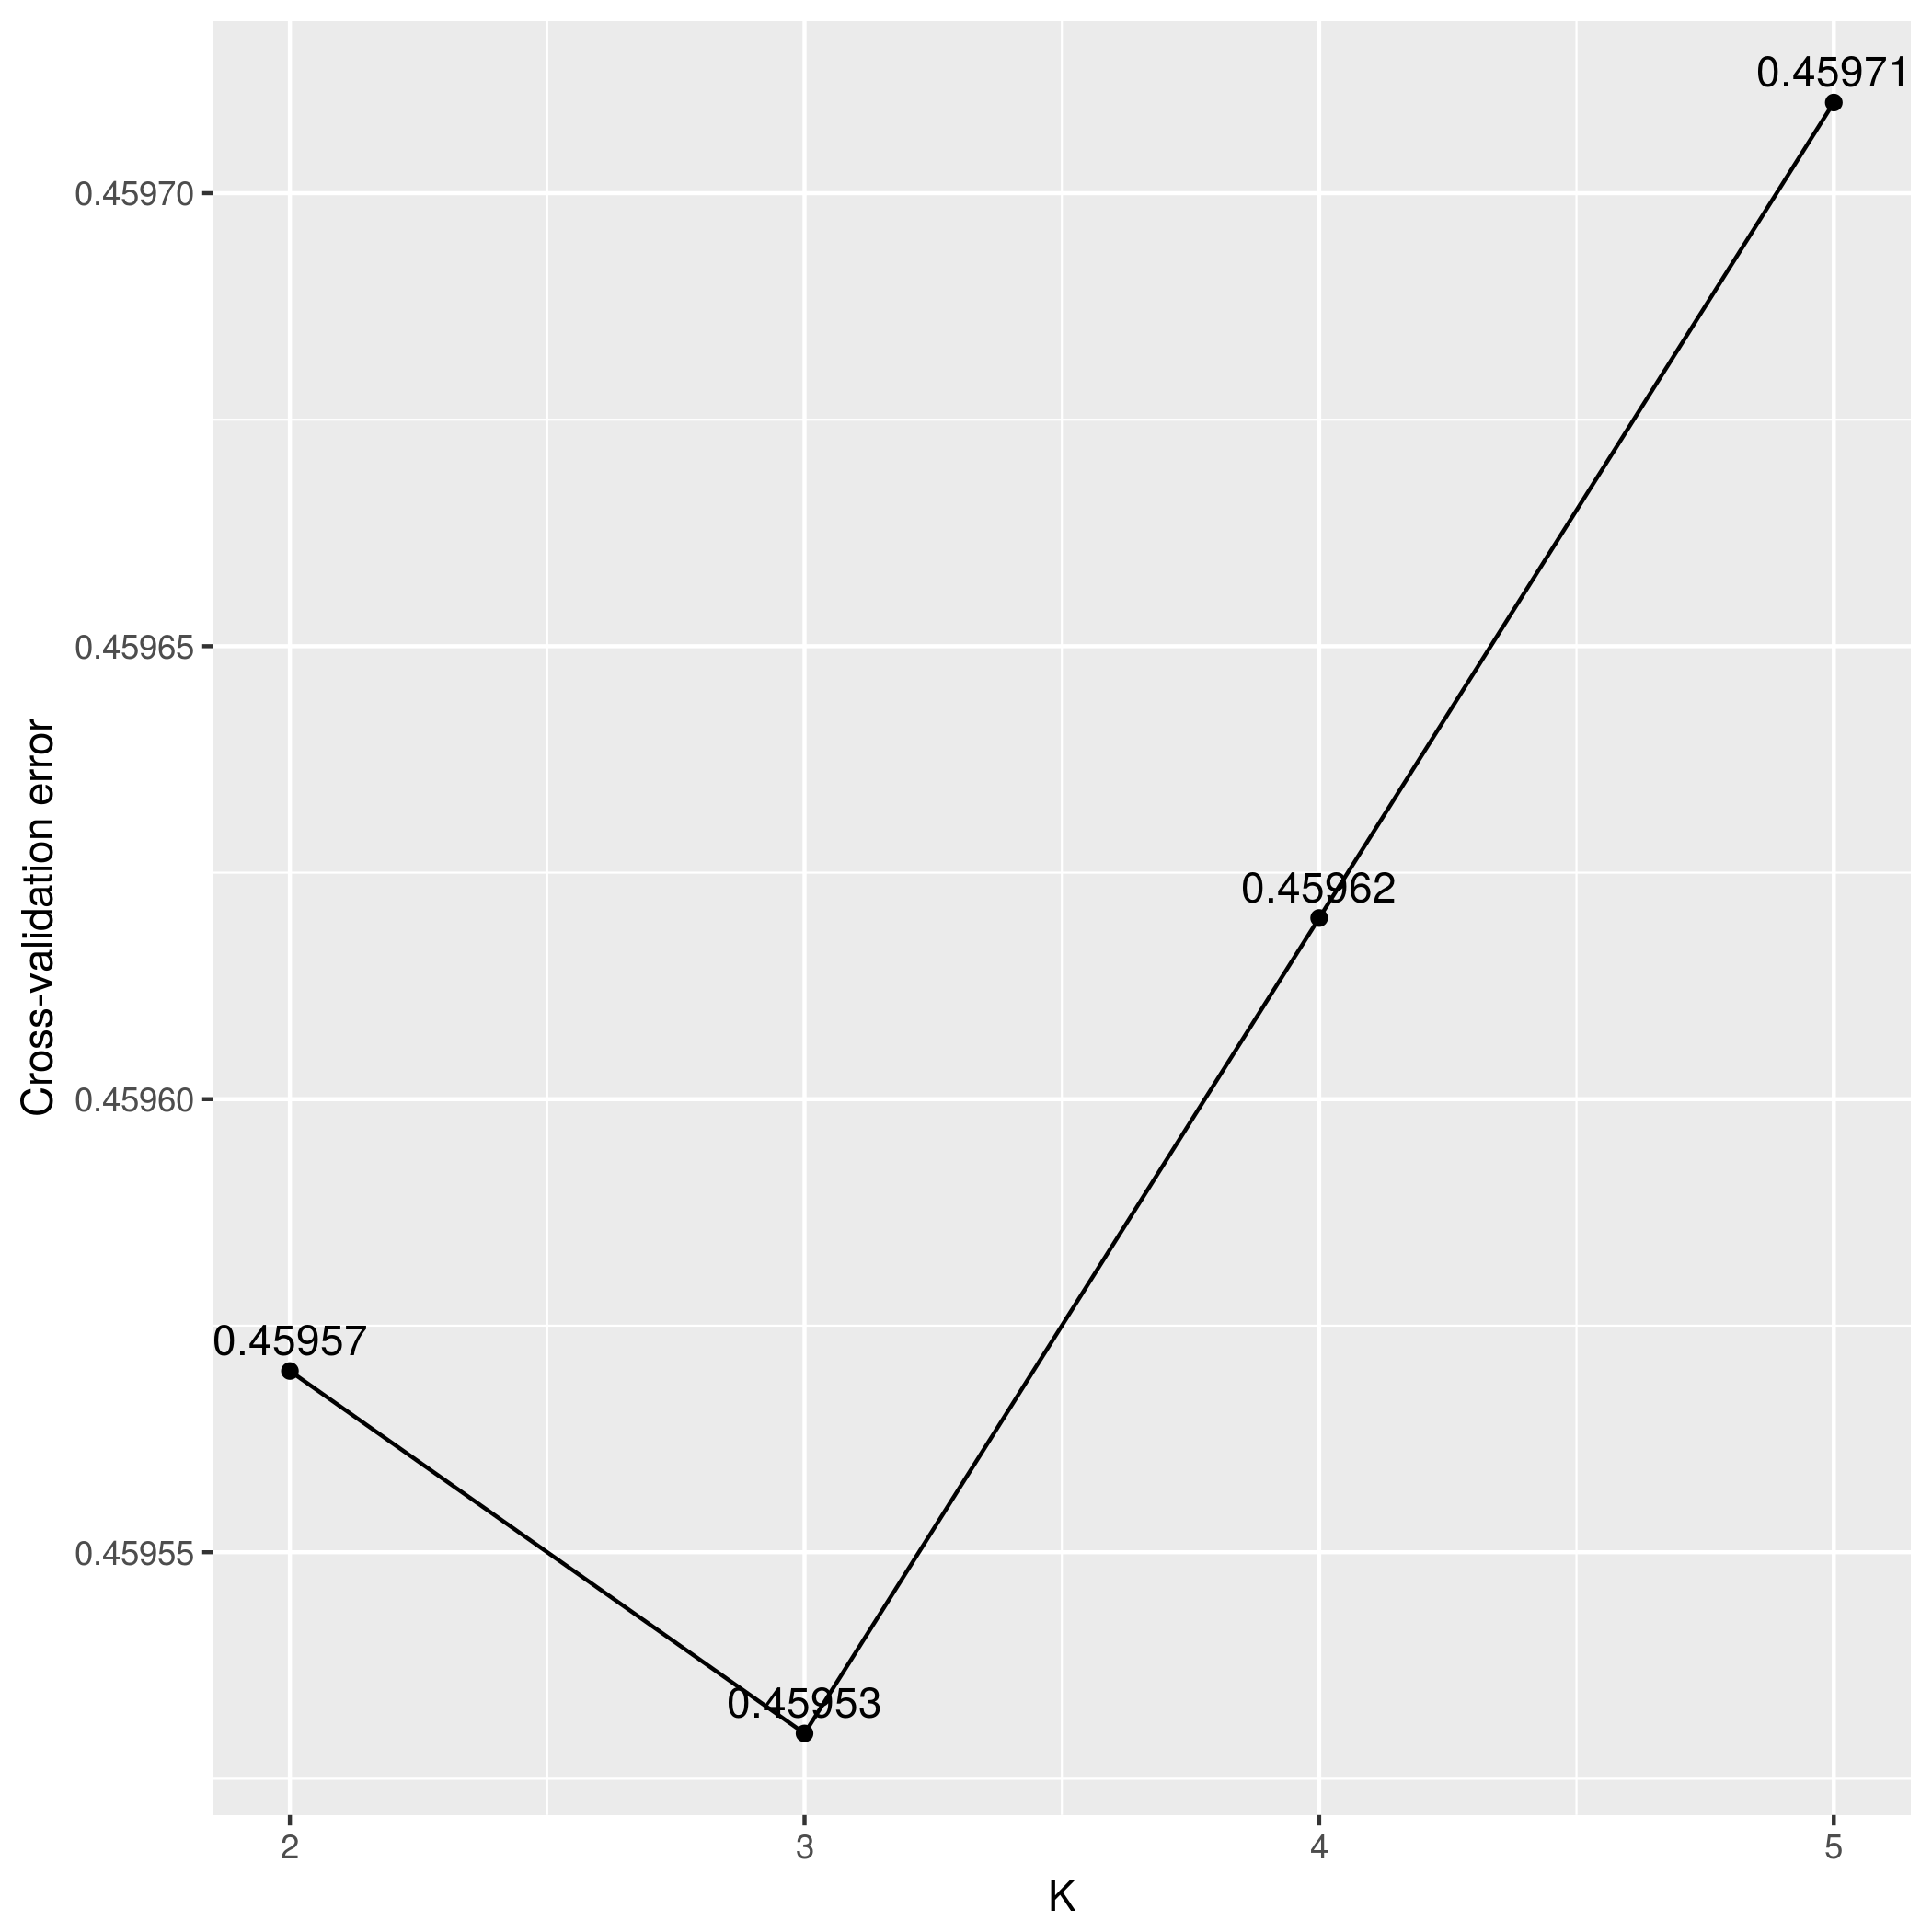
\includegraphics[scale=0.4]{K5.png}
  \caption{Error m\'etodo de cross-validation}
  \label{fig:crv}
\end{figure}
\end{frame}




\begin{frame}\frametitle{Gr\'afica de colores K=3}
    
 
\begin{figure}[H]
  \centering
  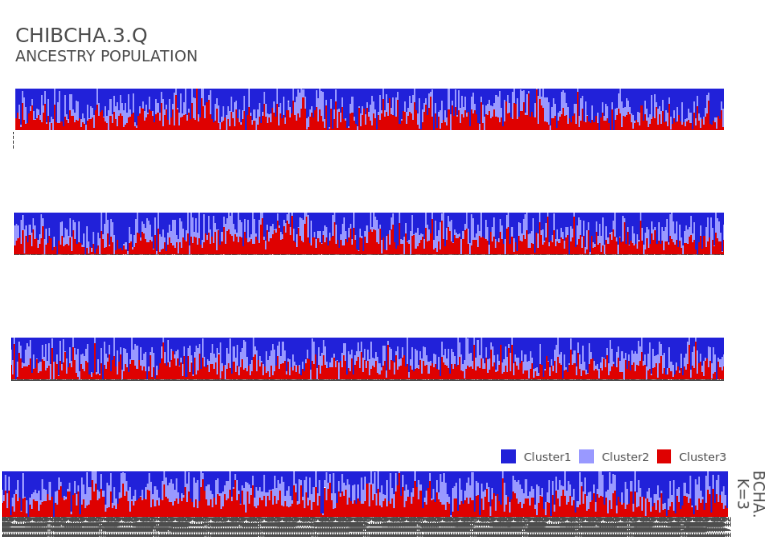
\includegraphics[scale=0.4]{K3.png}
  \caption{Gr\'afica de color de ancestria}
  \label{fig:crv}
\end{figure}
\end{frame}


\begin{frame}\frametitle{Relacionando los cluster con poblaci\'on geografica}

  Para relacionar los colores con poblaciones se requiere correr el proyecto HAPMAP. El objetivo del Proyecto Internacional HapMap era crear un mapa de haplotipos del genoma humano. A menudo conocido como el HapMap, éste describe los patrones comunes de la variación genética humana.

El HapMap proporciona un recurso clave que los investigadores pueden usar para encontrar genes que afectan a la salud, la enfermedad y las respuestas a los medicamentos y los factores ambientales. La información producida por el proyecto está ahora disponible gratuitamente en bases de datos públicas a los investigadores alrededor del mundo.
\end{frame}

\begin{frame}\frametitle{Relacionando los cluster con poblaci\'on geografica}
  Las siguientes muestras de poblaciones fueron estudiadas en este proyecto:

\begin{verbatim}
ASW African ancestry in Southwest USA

CEU Utah residents with Northern and Western European ancestry from the CEPH collection

CHB Han Chinese in Beijing, China

CHD Chinese in Metropolitan Denver, Colorado

GIH Gujarati Indians in Houston, Texas

JPT Japanese in Tokyo, Japan

LWK Luhya in Webuye, Kenya

MXL Mexican ancestry in Los Angeles, California

MKK Maasai in Kinyawa, Kenya

TSI Toscani in Italia

YRI Yoruba in Ibadan, Nigeria 
\end{verbatim}
\end{frame}

\begin{frame}\frametitle{TAREAS POR REALIZAR}
   \begin{itemize}
   \item Asociar las regiones de los SNP's con la ancestralidad de los individuos. \texttt{En proceso - 80\%}
   \item Asociar los SNP's que tienen relacio\'on con el CCR y observar su procedencia de ascedencia.
  \end{itemize}

\end{frame}



\section{Referencias}
\begin{frame}[fragile]\frametitle{Referencias}
  \bibliographystyle{acm}
  \bibliography{Bibliografia/biblio}  
\end{frame}



\begin{frame}[fragile]\frametitle{}

\begin{center}
  GRACIAS
\end{center}
\end{frame}










\end{document}
